\section{Experimental Results and Discussion}\label{sec:experiments}

\subsection{Experimental Setup and Baselines}
All predictive models are trained strictly on full-year 2024 TDCS M05A telemetry across the 10 Freeway No.~5 mainline segments. Evaluation is performed chronologically on two unseen periods: (1) the full 2025 test year (365 days: 247 weekdays, 87 regular weekends, 31 long-holiday days) and (2) an out-of-sample 2026 period from January~1 to November~8, 2026 (311 days: 206 weekdays, 73 regular weekends, 32 long-holiday days). Probability calibrators are fitted on 2025~H1 and evaluated on 2025~H2 and 2026.

We compare our \texttt{HistGradientBoosting} model (GBM) against two strong, transparent baselines:
\begin{itemize}
    \item \textbf{Persistence:} Predicts $\hat{v}_k(t+h) = v_k(t)$ (current speed persists). Any short-term model must first beat persistence.
    \item \textbf{Historical Average (HA):} Lookup mean speed by segment, time-of-day slot, and calendar day type computed on 2024 training data (no real-time input).
\end{itemize}
Because 5-minute samples within the same day are strongly autocorrelated, all 95\% confidence intervals (CIs) are computed via day-level block bootstrap with paired differences between methods. Software reproducibility is backed by 40 unit tests (\texttt{pytest}) covering alignment, stale-data refusal, rule parsing, knowledge-base filtering, and numerical verification.

\subsection{Speed Prediction Accuracy}
Table~\ref{tab:mae} and Fig.~\ref{fig:mae} report speed Mean Absolute Error (MAE, in km/h) stratified by horizon and day type across 2025 and 2026. Three findings emerge:
\begin{enumerate}
    \item \textbf{Consistent gains on weekdays and regular weekends:} Across all three horizons and both years, GBM significantly outperforms both HA and Persistence. At the 60-minute horizon, weekday MAE drops from 3.77 to 3.02~km/h ($\Delta = -0.75$, 95\% CI [$-0.79, -0.70$]) in 2025 and from 3.66 to 3.11~km/h ($\Delta = -0.55$, [$-0.60, -0.50$]) in 2026. Regular-weekend 60-minute MAE improves by $-0.70$~km/h in 2025 and $-0.50$~km/h in 2026. HA performs poorly on weekends ($>8$~km/h) and holidays ($>9.8$~km/h) because it ignores live traffic states.
    \item \textbf{Fragile and small gains on long holidays:} Holiday improvements over persistence are substantially smaller and unstable across years. At 60~minutes, GBM reduces holiday MAE by $-0.31$~km/h ([$-0.41, -0.20$]) in 2025, but in 2026 the difference shrinks to $-0.04$~km/h with a 95\% CI of [$-0.17, +0.08$] spanning zero.
    \item \textbf{Modest absolute magnitude:} Even when statistically significant, absolute reductions over persistence range from $0.04$ to $0.75$~km/h relative to base MAEs of $2.5$--$4.9$~km/h. Consequently, any claim of forecasting superiority must be reported by day type, and our agent explicitly appends a holiday accuracy caveat whenever the queried date falls on a long holiday.
\end{enumerate}

\begin{table*}[t]
\caption{Speed Prediction MAE (km/h) and Paired Difference Against Persistence (GBM $-$ Persistence) with Day-Level Bootstrap 95\% Confidence Intervals}
\label{tab:mae}
\centering
\begin{tabular}{llcccccccc}
\toprule
\multirow{2}{*}{Horizon} & \multirow{2}{*}{Day Type} & \multicolumn{4}{c}{2025 Test Year (365 Days)} & \multicolumn{4}{c}{2026 Out-of-Sample (311 Days)} \\
\cmidrule(lr){3-6} \cmidrule(lr){7-10}
 & & HA & Persist. & GBM & $\Delta$ (95\% CI) & HA & Persist. & GBM & $\Delta$ (95\% CI) \\
\midrule
\multirow{3}{*}{15 min}
 & Weekday     & 4.18 & 2.60 & \textbf{2.22} & $-0.39$ [$-0.40, -0.38$] & 4.68 & 2.56 & \textbf{2.20} & $-0.36$ [$-0.38, -0.35$] \\
 & Weekend     & 8.12 & 2.84 & \textbf{2.51} & $-0.32$ [$-0.34, -0.30$] & 8.54 & 2.79 & \textbf{2.48} & $-0.31$ [$-0.34, -0.28$] \\
 & Holiday     & 9.87 & 2.72 & \textbf{2.53} & $-0.19$ [$-0.23, -0.15$] & 10.50 & 2.61 & \textbf{2.47} & $-0.14$ [$-0.18, -0.10$] \\
\midrule
\multirow{3}{*}{30 min}
 & Weekday     & 4.19 & 3.03 & \textbf{2.56} & $-0.47$ [$-0.49, -0.46$] & 4.70 & 2.96 & \textbf{2.56} & $-0.40$ [$-0.43, -0.38$] \\
 & Weekend     & 8.20 & 3.59 & \textbf{3.20} & $-0.40$ [$-0.45, -0.35$] & 8.61 & 3.50 & \textbf{3.16} & $-0.34$ [$-0.39, -0.29$] \\
 & Holiday     & 9.97 & 3.37 & \textbf{3.19} & $-0.18$ [$-0.23, -0.14$] & 10.59 & 3.23 & \textbf{3.17} & $-0.06$ [$-0.11, -0.01$] \\
\midrule
\multirow{3}{*}{60 min}
 & Weekday     & 4.22 & 3.77 & \textbf{3.02} & $-0.75$ [$-0.79, -0.70$] & 4.74 & 3.66 & \textbf{3.11} & $-0.55$ [$-0.60, -0.50$] \\
 & Weekend     & 8.35 & 4.85 & \textbf{4.15} & $-0.70$ [$-0.81, -0.58$] & 8.77 & 4.71 & \textbf{4.21} & $-0.50$ [$-0.62, -0.38$] \\
 & Holiday     & 10.15 & 4.44 & \textbf{4.13} & $-0.31$ [$-0.41, -0.20$] & 10.78 & 4.28 & 4.24 & $-0.04$ [$-0.17, +0.08$] \\
\bottomrule
\end{tabular}
\end{table*}


\begin{figure*}[t]
\centering
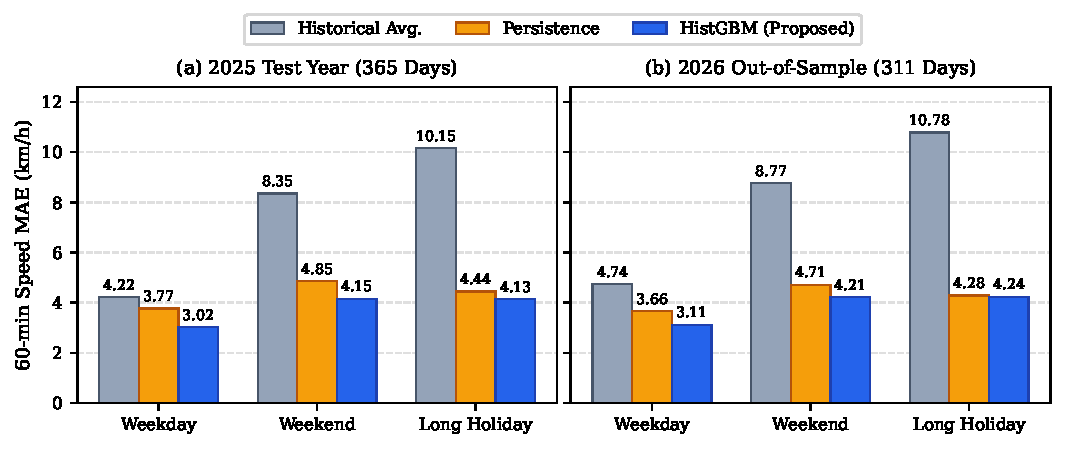
\includegraphics[width=0.92\textwidth]{mae_comparison.pdf}
\caption{Comparison of 60-minute speed prediction MAE (km/h) across day types for (a) the 2025 test year and (b) the 2026 out-of-sample period. While HistGBM consistently beats Persistence on weekdays and weekends, holiday gains are marginal in 2025 and statistically indistinguishable from zero in 2026.}
\label{fig:mae}
\end{figure*}

\subsection{Event-Level Early-Warning Evaluation}
Although sample-level congestion ROC-AUC appears very high (in 2026 out-of-sample data across $>637{,}000$ slots: 0.997 at 15~min, 0.993 at 30~min, and 0.986 at 60~min with only $\approx 2.6\%$ positive rate), sample-level metrics are dominated by prolonged already-congested or free-flow regimes and cannot measure \textit{advance warning}.

We therefore evaluate true early warning under a strict event-level protocol: alerts are evaluated \textit{only} when traffic is currently free-flowing ($v_k \ge 40$~km/h over the last 30~min); consecutive alerts on the same segment within 30~min are merged; thresholds are matched to fixed alert budgets of $0.25$, $0.50$, and $1.00$ alerts/segment/day; and an event is counted as detected if an alert fires within 60~min before onset (precision counts alerts followed by an event within 60~min).

Table~\ref{tab:events} and Fig.~\ref{fig:events} reveal a critical negative finding:
\begin{itemize}
    \item \textbf{Deployed classifier underperforms persistence:} At the low-noise 0.25 alert budget, the deployed classifier achieves only 0.42 detection (0.42 precision) in 2025 and 0.26 detection (0.23 precision) in 2026, trailing simple Persistence (0.70 / 0.73 in 2025; 0.76 / 0.71 in 2026) with non-overlapping CIs.
    \item \textbf{Dedicated onset model fails pre-registered deployment gate:} We trained a specialized \texttt{Onset} classifier exclusively on free-flow samples using speed-trend, recent-minimum, and volume-change features. While it closed the gap and slightly beat Persistence at the 0.50 budget ($+0.038$ [$+0.023, +0.053$] in 2025; $+0.031$ [$+0.018, +0.045$] in 2026), it failed our pre-registered success criterion requiring the 95\% CI lower bound to exceed zero at \textit{both} 0.25 and 0.50 budgets in 2025 (at 0.25: $+0.032$ [$-0.004, +0.070$]; on 2026 holidays at 0.50: $+0.000$ [$-0.047, +0.052$]). Adhering to our pre-registered gate, we did \textit{not} integrate the Onset model into the agent and explicitly frame calibrated probabilities as relative risk indicators rather than early-warning alarms.
\end{itemize}

\begin{table}[t]
\caption{Event-Level Early-Warning Detection Rate / Precision Under Fixed Alert Budgets (Alerts per Segment per Day)}
\label{tab:events}
\centering
\setlength{\tabcolsep}{4pt}
\begin{tabular}{llccc}
\toprule
Period & Method & 0.25 & 0.50 & 1.00 \\
\midrule
\multirow{4}{*}{\shortstack[l]{2025 Full\\(918 events)}}
 & Persistence & 0.70 / 0.73 & 0.91 / 0.48 & 0.96 / 0.26 \\
 & Hist. Avg.  & 0.36 / 0.37 & 0.61 / 0.32 & 0.97 / 0.25 \\
 & Deployed Clf. & 0.42 / 0.42 & 0.84 / 0.43 & 0.97 / 0.25 \\
 & Onset Model$^{\dagger}$ & \textbf{0.73 / 0.75} & \textbf{0.95 / 0.48} & \textbf{0.97 / 0.25} \\
\midrule
\multirow{4}{*}{\shortstack[l]{2026 Full\\(680 events)}}
 & Persistence & 0.76 / 0.71 & 0.94 / 0.43 & 0.96 / 0.22 \\
 & Hist. Avg.  & 0.34 / 0.39 & 0.65 / 0.29 & 0.99 / 0.22 \\
 & Deployed Clf. & 0.26 / 0.23 & 0.83 / 0.37 & 0.98 / 0.22 \\
 & Onset Model$^{\dagger}$ & \textbf{0.79 / 0.70} & \textbf{0.97 / 0.43} & \textbf{0.98 / 0.22} \\
\bottomrule
\multicolumn{5}{l}{\footnotesize $^{\dagger}$Not integrated into Agent: failed pre-registered 0.25-budget CI criterion.}
\end{tabular}
\end{table}


\begin{figure}[t]
\centering
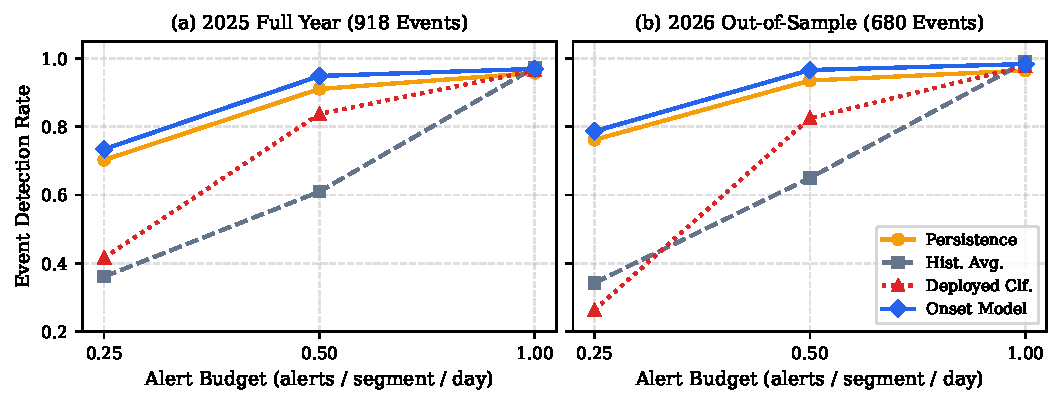
\includegraphics[width=\columnwidth]{event_warning.pdf}
\caption{Event-level early-warning detection rate under fixed alert budgets (0.25, 0.50, 1.00 alerts/segment/day) for (a) 2025 and (b) 2026. The deployed classifier trails Persistence at low alert budgets, illustrating the pitfalls of relying on sample-level AUC.}
\label{fig:events}
\end{figure}

\subsection{Probability Calibration and Data Latency Robustness}
On 2025~H2 free-flow samples with predicted congestion risk $\ge 0.3$, grouped isotonic calibration reduced the absolute gap between mean predicted probability and observed congestion frequency from $0.263 \rightarrow 0.082$ (15~min), $0.165 \rightarrow 0.042$ (30~min), and $0.034 \rightarrow 0.028$ (60~min), satisfying our pre-registered target ($\le 0.10$ across all horizons). However, on out-of-sample 2026 data (where positives cluster on fewer days), calibrated high-risk bins remained overestimated by roughly $2\times$ (e.g., 30-min mean predicted $0.45$ vs.\ observed $0.24$), confirming that probabilities should be communicated as qualitative risk levels rather than exact frequencies.

To assess operational resilience under feed delays, we simulated decision-time telemetry lags of $0, 5, 10,$ and $15$~minutes on 2025 data without retraining. At the 60-minute horizon, GBM MAE increased gradually from $3.39$ to $3.59$~km/h (approximately $+0.1$~km/h per 5-minute delay), whereas Persistence degraded from $4.09$ to $4.49$~km/h; thus, a 15-minute-delayed GBM still outperformed zero-delay Persistence.

\subsection{End-to-End Agent Evaluation}
We evaluated the complete agent across 72 frozen test cases (60 core cases covering normal queries, out-of-scope refusals, missing-slot clarifications, directional inference, announcement matching, missing data, and tool failures, plus 12 live-mode, open-phrasing, and holiday-caveat cases), executed 3 times per case in both Template and LLM (\texttt{qwen/qwen3-14b}) modes. Results are summarized in Table~\ref{tab:agent}.

Both modes achieved 100\% across all deterministic guardrail checks, including zero numerical hallucinations, exact announcement citations, and 3-run consistency. In LLM mode, approximately 86\% of responses were accepted directly, while the remaining 14\% triggered safe fallback to the deterministic template due to numerical or required-content verification failures. Median latency was $\approx 2$~s in Template mode and $9$--$14$~s (p95: $20$--$24$~s) in LLM mode.

Critically, we caution against over-interpreting these 100\% automated scores: because test phrasings mirror rule patterns and core decisions are deterministic, automated metrics verify regression safety rather than natural-language quality under unconstrained user queries. Indeed, prior to adding programmatic post-appending, the LLM voluntarily included the holiday caveat in only 40\% (31/78) of holiday runs---a defect invisible until explicitly encoded into both deterministic post-processing and scoring rubrics. Formal human evaluation of readability and helpfulness remains future work.

\begin{table}[t]
\caption{End-to-End Agent Evaluation Across 72 Frozen Cases (3 Runs Each, Total 216 Executions per Mode)}
\label{tab:agent}
\centering
\begin{tabular}{lcc}
\toprule
Metric & Template Mode & LLM Mode (\texttt{qwen3-14b}) \\
\midrule
Refusal \& Clarification Accuracy & 100\% & 100\% \\
Zero Numerical Hallucination & 100\% & 100\% \\
Announcement Citation Accuracy & 100\% & 100\% \\
Advisory-Rule Consistency & 100\% & 100\% \\
Holiday Caveat Inclusion & 100\% & 100\%$^{\ddagger}$ \\
3-Run Consistency & 100\% & 100\% \\
LLM Output Adoption Rate & --- & $\approx$86\% (14\% fallback) \\
Median Latency (p50) & $\approx$2 s & 9--14 s (p95: 20--24 s) \\
\bottomrule
\multicolumn{3}{l}{\footnotesize $^{\ddagger}$40\% (31/78) when left to LLM; 100\% after deterministic post-append.}
\end{tabular}
\end{table}

